To exemplify the usefulness of such translations across libraries, we will examine one example with computer algebra systems -- which the \ODK research community has come to call \emph{Jane's Use Case}~\cite{ODK:interop:17} -- in detail. This example is interesting in that it was (chiefly) developed by John Cremona as a real-world situation a computational group theorist might find themself in, and where they would want to use a combination of computer algebra systems.

A user, Jane, wants to experiment with invariant theory of finite groups. She does so, by considering some group $G$ as acting on the variables $X_1,\ldots, X_n$ of the polynomial ring $\mathbb Z[X_1,\ldots,X_n]$ and studying the ideals generated by the orbit of some polynomial, since these happen to be fixed by the group action. Naturally, in a computational setting one would want to have the Gröbner bases of these ideas as well. \GAP happens to be efficient in computing orbits, whereas \Singular is known to be very efficient in computing Gröbner bases. For the purposes of this section (and in light of \autoref{sec:import:cas}) we will substitute \Singular by \Sage.

Starting from the Math-in-the-Middle ontology (see \autoref{sec:lf:mitm}), Jane wants to study the dihedral group $D_4$. So she declares a polynomial $p$ -- exemplary $3X_1+2X_2$ -- over $R=\mathbb{Z}[X_1,X_2,X_3,X_4]$, and wants to compute the orbit $O(\mathbb Z,D_4,p)$ in \GAP, translate the resulting ideal back to MitM as $I$, declare its Gröbner base $G=\mathtt{Groebner}(\mathbb Z,I)$, translate this to \Sage in order to compute it and have the result presented to her back in MitM.\medskip

There are two things that make this example particularly non-trivial:
\begin{enumerate}
	\item The terminologies employed by \GAP and \Sage differ: The dihedral group of order 8 is called $D_4$ in Sage, and $D_8$ in \GAP; the conversion between the two is not easily expressed in a single alignment.
	\item The ways polynomials are constructed in \GAP and \Sage differ considerably. 
	
	The polynomial $3X_1+2X_2$ is formally constructed in \GAP using the (internal) syntax
		\[\expr{ Poly_{\GAP}(RationalFunctions(FamilyObject(1)),[[1,1],3,[2,1],2])},\]
		where $[\ldots]$ represents lists, and $[[k_1,n_1,\ldots,k_m,n_m],a]$ represents the monomial $aX_{k_1}^{n_1}\cdot\ldots\cdot X_{k_m}^{n_m}$. The precise meaning of the \expr{FamilyObject} and \expr{RationalFunctions} symbols is technical and largely irrelevant.
		
		In \Sage, the same polynomial is instead constructed as 
		\[ \expr{ Poly_{\Sage}(PolyRing(\mathbb Z,[X_1,X_2,X_3,X_4]),[[[1,0,0,0],3],[[0,1,0,0],2]])}, \]
		where $[[i_1\ldots i_n],a]$ represents the monomial $aX_1^{i_1}\cdot\ldots\cdot X_n^{i_n}$. Consequently, monomials refer to the specific named variables of the polynomial ring $\mathbb Z[X_1,X_2,X_3,X_4]$ provided as an argument.
		
		In general and not surprisingly, there seems to be no universally agreed upon method to formally represent polynomials. 
\end{enumerate}

The symbols for lists, integers, Gröbner bases, ideals (which in a computational setting can be represented as a list of generators) and orbits can be easily expressed as typed constants in an interface theory and connected via alignments, so we can focus on those aspects of the translation that are non-trivial.

The discrepancy regarding dihedral groups is reflective of different notational conventions used in the mathematical community, hence it makes sense to have both of them represented in an interface. Correspondingly, for the interface theory in the Math-in-the-Middle library we use both and simply use definitions to convert between them:

\begin{mmtcode}[caption= {An Interface Theory for Dihedral Groups},label=fig:crosslib:dihedraltheory]
theory Dihedral :base:?Logic =
	dihedralD 	: ℕ+ → group ❙
	dihedral 	: ℕ+ → group ❘ = [z] dihedralD (2 ⋅ z) ❙
\end{mmtcode}
Which allows us to use simple alignments to translate from \GAP/\Sage to MitM and definition expansion to translate from the second to the first variant. For the other direction, we need a theory morphism, e.g. a view:
\begin{mmtcode}[caption= {An View for Translating Dihedral Groups},label=fig:crosslib:dihedralview]
view DihedralTranslation : ?Dihedral -> ?Dihedral =
	dihedralD = [n] dihedral (n / 2) ❙
\end{mmtcode}

Regarding converting polynomials, we are stuck with using a programmatic translator instead. For a MitM representation of polynomials, we use a more generic method that carries the names of the variables:
\begin{mmtcode}[caption= {An Interface Theory for Integer Polynomials\protect\footnotemark},label=fig:crosslib:mitmpoly]
theory Polynomials : base:?Logic =
	polynomialRing : ring ⟶ type ❙
	monomial : ring ⟶ type ❘ # monomial 1❙
	multi_poly_con : {r : ring} List (monomial r) ⟶ multi_polynomial r ❘ # mpoly 2 ❙
	monomial_con : {r: ring} (List (string × ℕ)) × r.universe ⟶ monomial r ❘ # monomial_con 1 2❙
❚

theory IntegerPolynomials : base:?Logic =
	include ?Polynomials ❙
	include algebra?IntegerRing ❙
	int_polynomial : List (monomial ℤ) ⟶ multi_polynomial ℤ ❙
	int_monomial : (List (string × ℕ)) × ℤ ⟶ monomial ℤ ❙
❚
\end{mmtcode}
\footnotetext{Adapted and simplified from \url{https://gl.mathhub.info/MitM/smglom/blob/master/source/algebra/polynomials.mmt}}

The polynomial $3X_1+2X_2$ would then be represented as 
\[\expr{int\_polynomial([int\_monomial(\pair{[\pair{\text{``}X1\text{''}}1]}{3}),int\_monomial(\pair{[\pair{\text{``}X2\text{''}}1]}{2})])}.\]

\paragraph{} The only thing missing then are programmatic translators from \GAP and \Sage to MitM and their inverses. As an example, \autoref{lst:crosslib:polytrans} shows the translator from MitM polynomials to \GAP polynomials, using helper objects (analogous to those described in \autoref{sec:lf:lfx:sigma:symbolrefs}).
\begin{scalacode}[caption= {A Translator from MitM Polynomials to \GAP{\protect\footnotemark}},label=lst:crosslib:polytrans]
val toPolynomials = new AcrossLibraryTranslation {
    def applicable(tm: Term): Boolean = tm match {
      case MitM.MultiPolynomial(_,_) => true
      case _ => false
    }
    def apply(tm: Term): Term = tm match {
      case MitM.MultiPolynomial(_,ls) =>
        Poly(ls.flatMap{
          case (vars,coeff,_) =>
            LFList(vars.flatMap(p => List(Integers(variables.get(p._1)),Integers(p._2)))) :: Integers(coeff) :: Nil
        })
    }
  }
\end{scalacode}
\footnotetext{https://github.com/UniFormal/MMT/blob/master/src/mmt-odk/src/info/kwarc/mmt/odk/GAP/GAPSystem.scala}

Given these translators, Jane's Use Case can be realized as a sequence of applications of the translation algorithm described in \autoref{sec:crosslib:translate:impl}. 

\autoref{fig:crosslib:trans:jupyter} shows the realization of this use case in a Jupyter~\cite{jupyter-project:on} notebook running an \mmt kernel. Here, the expression $\expr{Evaluate(S,t)}$ is used to instruct the \mmt system to translate the expression $t$ to the ontology of system $S$ and have the target system evaluate the expression.

\begin{figure}[ht]
  \begin{framed}
  	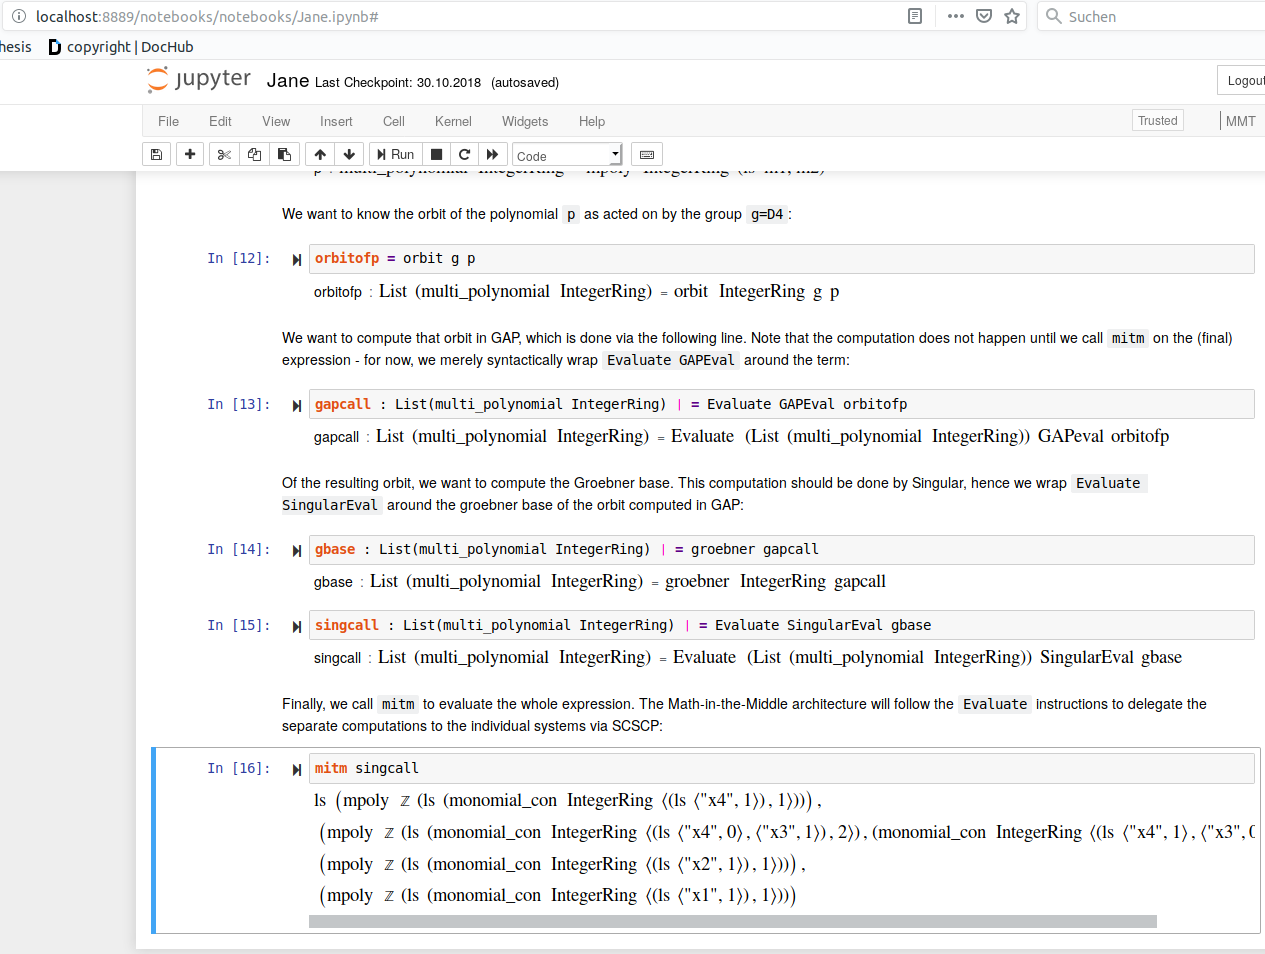
\includegraphics[width=\textwidth]{img/jupyter}
  \end{framed}
  \caption{Jane's Use Case in an \mmt Jupyter Notebook}\label{fig:crosslib:trans:jupyter}
\end{figure}